\documentclass[tikz,border=4pt]{standalone}
\usepackage{tikz}
\usetikzlibrary{arrows.meta,positioning}
\definecolor{nebula}{HTML}{6366F1}
\definecolor{spark}{HTML}{14B8A6}
\begin{document}
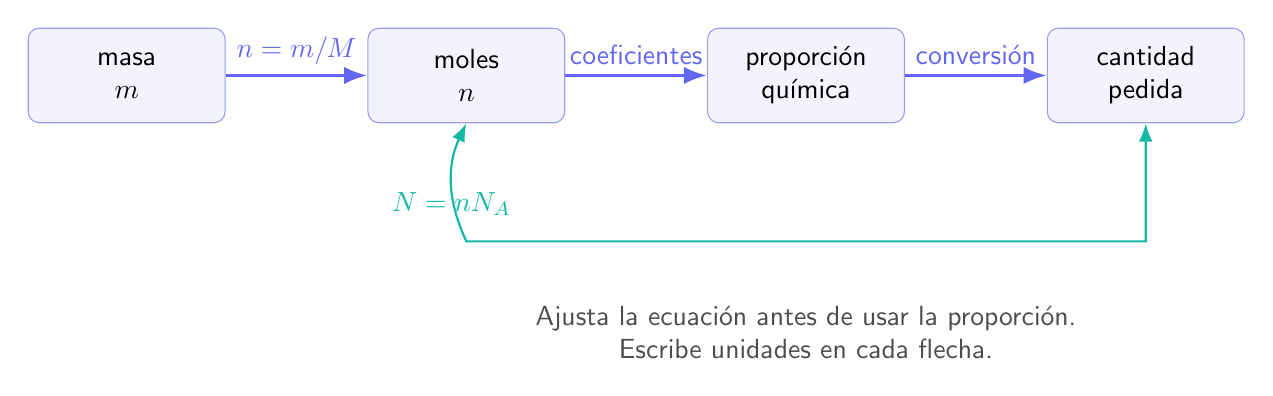
\begin{tikzpicture}[font=\sffamily,>=Latex,node distance=18mm]
  \tikzset{box/.style={rounded corners=4pt,draw=nebula!65,fill=nebula!8,minimum width=25mm,minimum height=12mm,align=center}}
  \node[box] (mass) {masa\\$m$};
  \node[box,right=of mass] (mol) {moles\\$n$};
  \node[box,right=of mol] (ratio) {proporci\'on\\qu\'imica};
  \node[box,right=of ratio] (target) {cantidad\\pedida};
  \draw[->,very thick,nebula] (mass)--node[above] {$n=m/M$} (mol);
  \draw[->,very thick,nebula] (mol)--node[above] {coeficientes} (ratio);
  \draw[->,very thick,nebula] (ratio)--node[above] {conversi\'on} (target);
  \draw[<->,thick,spark] (mol.south) to[bend right=25] node[below] {$N=nN_A$} ++(0,-1.5) -| (target.south);
  \node[below=22mm of ratio,align=center,text=black!70] {Ajusta la ecuaci\'on antes de usar la proporci\'on.\\Escribe unidades en cada flecha.};
\end{tikzpicture}
\end{document}
